\section{Future work \label{sec:Fut}}

\subsection{Autoinducer derivatives}

\begin{figure}[H]
	\begin{center}
		\schemeref[HHQaz]{cmpd:HHQaz}
		\schemeref[PQSaz]{cmpd:PQSaz}
		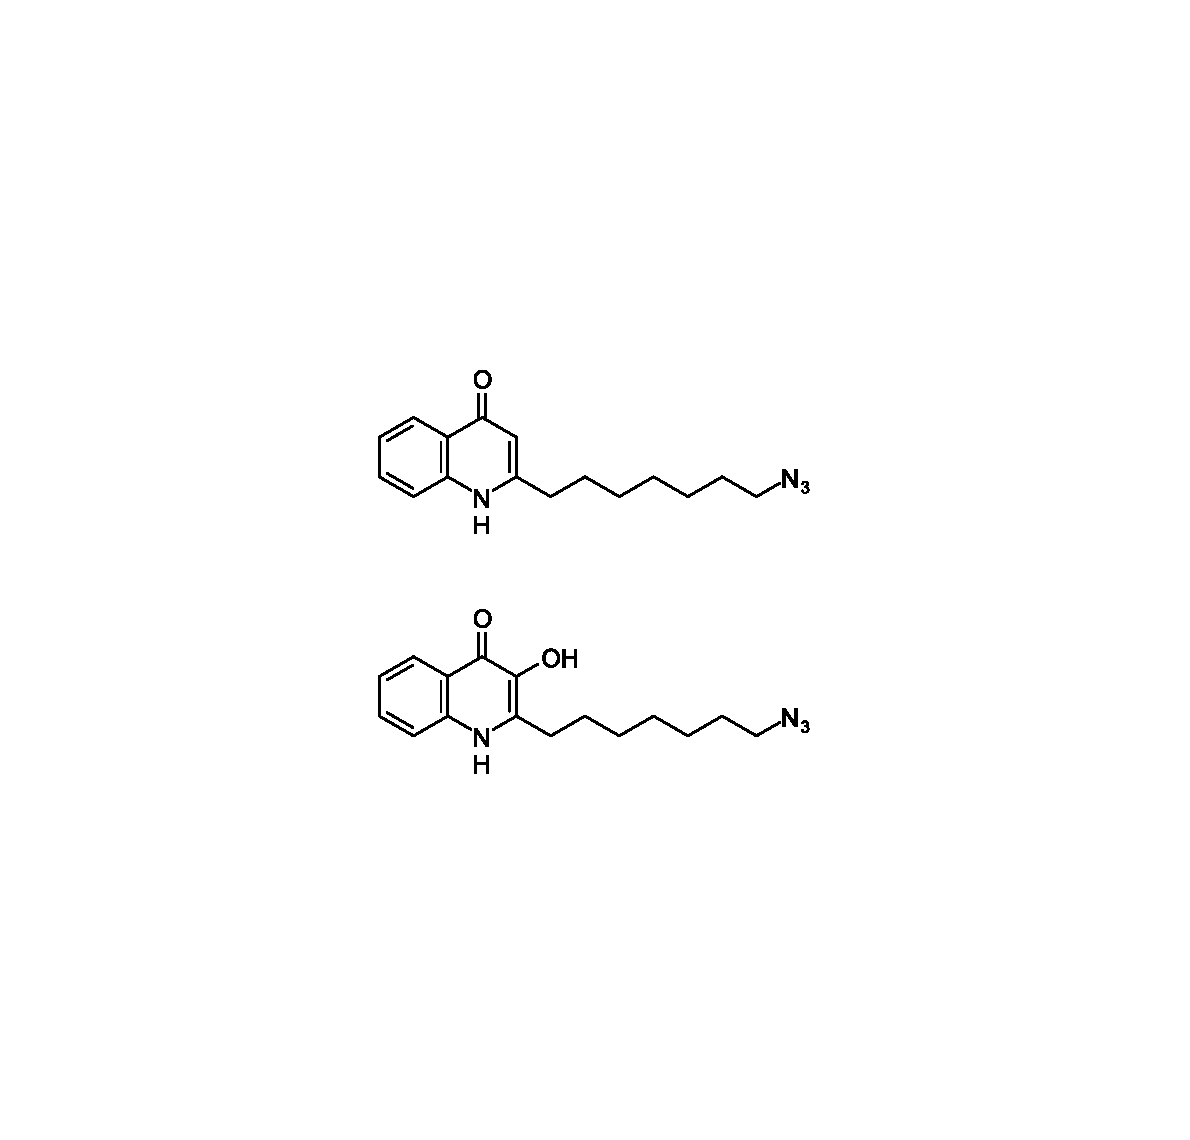
\includegraphics[scale=1]{HHQPQSaz}
		\caption{Further azido-HHQ \compound{cmpd:HHQaz} and azido-PQS \compound{cmpd:PQSaz} derivatives synthesised by Baker.\label{fgr:HHQPQSaz}} 
	\end{center}
\end{figure}

The syntheses of HHQ derivative \compound{cmpd:azHHQ} and azido-C$_4$-HSL derivative \compound{cmpd:HL4N3} will be completed as outlined above (see \ref{sec:azHHQ} and \ref{sec:HL4N3}). 
The only \textit{P. aeruginosa} autoinducer not yet to have been considered in this project is 3-oxo-C$_12$-HSL derivative \compound{cmpd:HLO12} (see \ref{fgr:PA_autoinducers}). This would be the most obvious next target for study. After this, there are several other autoinducers which are not produced by \textit{P. aeruginosa} which could be investigated (see \ref{fgr:autoinducers}) as we indend to screen the library against a range of bacteria.

\subsubsection{3-oxo-C$_12$-HSL derivative \compound{cmpd:HLO12N3} \label{sec:Fut_HLO12}}

The synthesis of 3-oxo-C$_12$-HSL has previously been reported by Hodgkinson \textit{et al.}\cite{Hodgkinson2011}. A modification of this synthesis using 10-bromodecanoyl chloride could be used to produce derivative \compound{cmpd:HLO12N3} with a tail azide (see \ref{sch:HLO12N3_synth}). Derivatives with shorter or longer tail lengths (known to affect selectivity and binding affinity) could also be synthesised using the same method. 

\begin{scheme}[H]
	\begin{center}
		\schemeref[HO10Br]{cmpd:HO10Br}
		\schemeref[HO10N3]{cmpd:HO10N3}
		\schemeref[Cl10N3]{cmpd:Cl10N3}
		\schemeref[MeOO12N3]{cmpd:MeOO12N3}
		\schemeref[MeOac12N3]{cmpd:MeOac12N3}
		\schemeref[HOac12N3]{cmpd:HOac12N3}
		\schemeref[HLHBr]{cmpd:HLHBr}
		\schemeref[HLac12N3]{cmpd:HLac12N3}
		\schemeref[HLO12N3]{cmpd:HLO12N3}
		\schemeref[HLO12N3]{cmpd:HLO12N3}
		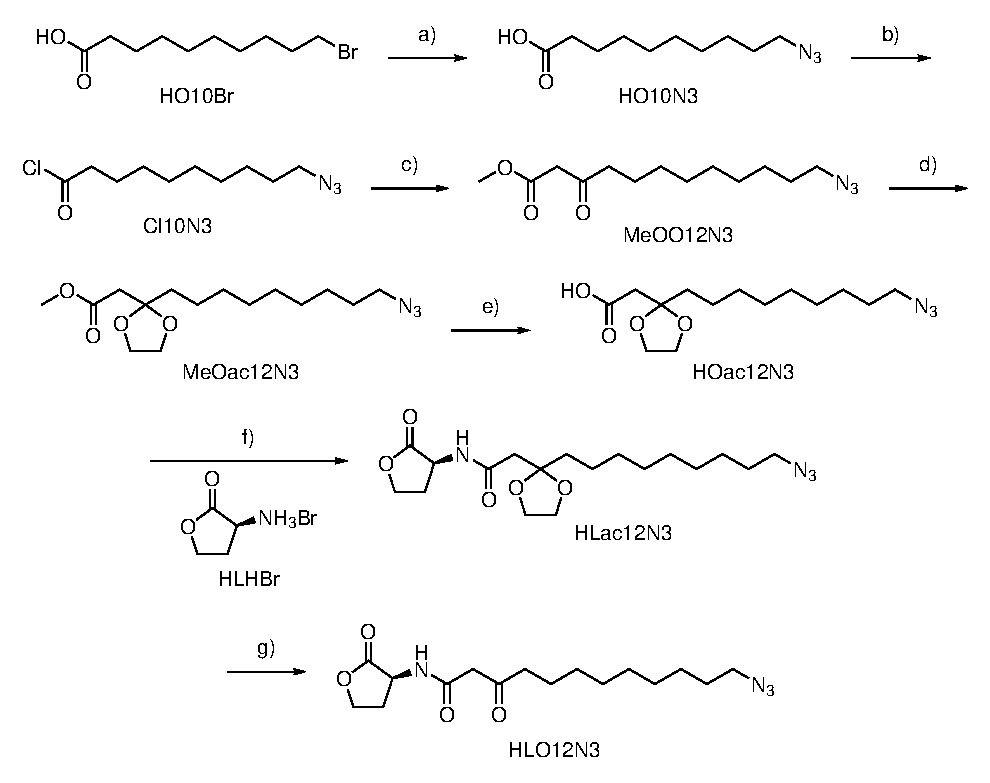
\includegraphics[scale=1]{HLO12N3_synth}
		\caption{Synthesis of azido 3-oxo-C$_12$-HSL derivative \compound{cmpd:HLO12N3} carried out by Ryan Howard.
		a) \ce{NaN3}, DMF, $50\ ^{\circ}$C.
		b) Oxalyl chloride, DMF, \ce{CH2Cl2}, r.t.
		c) MeOAc, \textit{N}-methyl imidazole, \ce{TiCl4}, DIPEA.
		d) \textit{p}-TsOH, \ce{HO(CH2)2OH}, \ce{CH(OMe)3}, r.t.
		e) NaOH, \ce{H2O}, r.t.
		f) EDC, DMAP, \ce{CH2Cl2}, r.t.
		g) TFA, r.t.
		\label{sch:HLO12N3_synth}}
	\end{center}
\end{scheme}

\subsubsection{AI2}

\subsubsection{Non-\textit{P. aeruginosa} autoinducers \label{sec:FutAIP}}

Many species of bacteria other than \textit{P. aeruginosa} produce autoinducers \cite{Praneenararat2012} (see \ref{fgr:autoinducers}). An azido derivative of C$_8$-HSL \compound{cmpd:HL8} could be produced in a similar manner to the C$_4$-HSL derivatives already synthesised. An azido derivative of 3-oxo-C$_6$-HSL \compound{cmpd:HLO6} could be produced in the manner proposed for 3-oxo-C$_12$-HSL \compound{cmpd:HLO12} above. Derivatives of AI-2 \compound{cmpd:AI2} could have azide groups in the place of the OH groups on the sugar section of the molecule. Derivatives of AIP \compound{cmpd:AIP} and ComX \compound{cmpd:ComX} could be synthesised by conversion of their terminal amines to azides.
Derivatives of AIP \compound{cmpd:AIP} could be produced by standard peptide synthesis methods with the inclusion of unnatural azido amino acids at different points along the peptide chain followed by formation of the thioester bond. ComX \compound{cmpd:ComX} contains a complex non-standard amino acid which would be time-consuming to synthesise, but if this could be achieved then peptide synthesis methods could also be used to introduce an azido amino within the peptide chain.

\begin{figure}[H]
	\begin{center}
		\schemeref[HL8]{cmpd:HL8}
		\schemeref[HLO6]{cmpd:HLO6}
		\schemeref[AI2]{cmpd:AI2}
		\schemeref[ComX1]{cmpd:ComX}
		\schemeref[AIP1]{cmpd:AIP}
		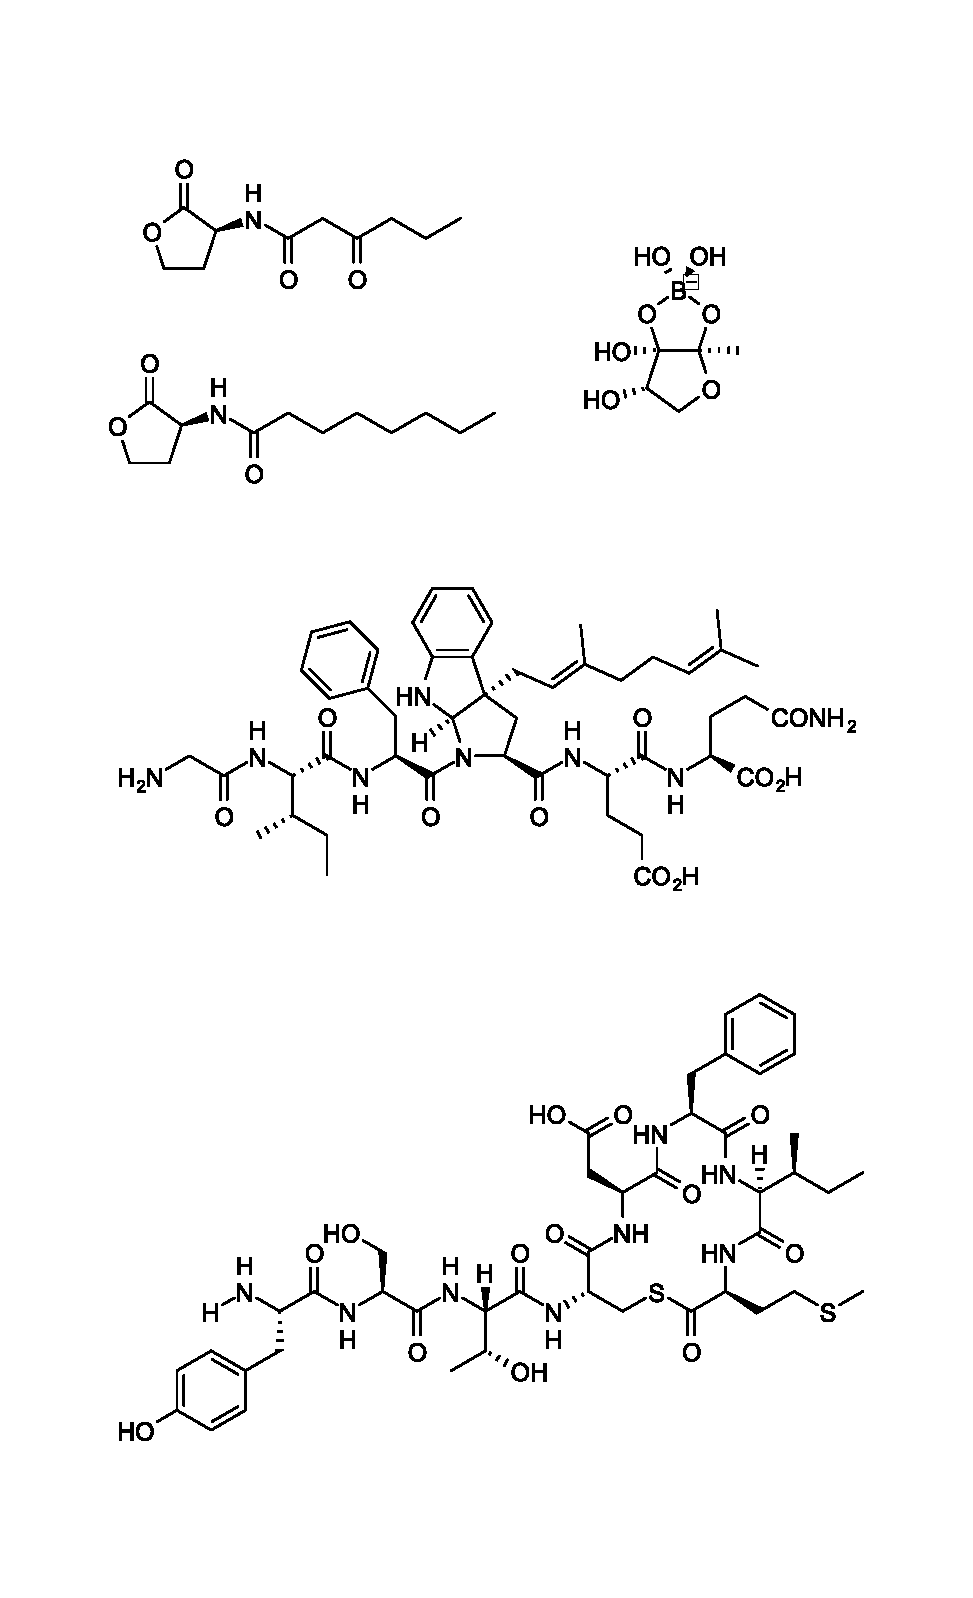
\includegraphics[scale=1]{QSMs}
		\caption{Autoinducers from various bacterial species. 
		C$_8$-HSL \compound{cmpd:HL8} is from \textit{Burkholderia cepacia}, 				
		3-oxo-C$_6$-HSL \compound{cmpd:HLO6} is from \textit{Erwinia chrysanthemi}, 
		AI-2 \compound{cmpd:AI2} is found in both Gram-positive and Gram-negative bacteria, 
		ComX \compound{cmpd:ComX} is from \textit{B. subtilis}, 
		AIP \compound{cmpd:AIP} is from \textit{S. aureus}.		
		\label{fgr:autoinducers}} 
	\end{center}
\end{figure}




\subsection{Antibiotic derivatives}

\subsubsection{Ciprofloxacin derivative \compound{cmpd:pipciphex}}

Derivative \compound{cmpd:pipciphex} has an alkyne tail attached in place of the cyclopropane ring at position 7 (see \ref{sch:cip_anas}); its retrosynthesis is shown in \ref{sch:pipciphex_retro}. This synthesis follows a conventional synthesis of ciprofloxacin similar to that reported by Mitscher \textit{et al.}\cite{Mitscher1986} but using hex-5-yn-1-amine \compound{cmpd:hexam} instead of cyclopropylamine. \compound{cmpd:24Cl5FbCl} should react with potassium ethyl malonate with loss of \ce{CO2} to form \compound{cmpd:24Cl5Fbke}, followed by heating with with triethyl orthoformate to form \compound{cmpd:24Cl5Fbkee}\cite{Mitscher1986, Senthilkumar2009}. This would then be heated with hex-5-yn-1-amine \compound{cmpd:hexam}, as opposed to the cyclopropylamine used in the conventional synthesis, to form \compound{cmpd:24Cl5Fbkeam}. Hex-5-yn-1-amine \compound{cmpd:hexam} could be produced using the Gabriel synthesis from \compound{cmpd:hexCl}\cite{Gabriel1887,Rozkiewicz2006,Pouy2012}. \compound{cmpd:24Cl5Fbkeam} could be cyclised using NaH to form \compound{cmpd:ClciphexEt} followed by ester hydrolysis using KOH to give \compound{cmpd:Clciphex} as reported by Mitscher \textit{et al.}. \compound{cmpd:Clciphex} would then be heated with piperazine in DMSO\cite{grohe19877} to complete the synthesis of \compound{cmpd:pipciphex}.

%\begin{scheme}[H]
%	\begin{center}
%		\schemeref[24Cl5FbCl]{cmpd:24Cl5FbCl}
%		\schemeref[24Cl5Fbke]{cmpd:24Cl5Fbke}
%		\schemeref[24Cl5Fbket]{cmpd:24Cl5Fbket}
%		\schemeref[24Cl5Fbkee]{cmpd:24Cl5Fbkee}
%		\schemeref[hexCl]{cmpd:hexCl}
%		\schemeref[hexphth]{cmpd:hexphth}
%		\schemeref[hexam]{cmpd:hexam}
%		\schemeref[24Cl5Fbkeam]{cmpd:24Cl5Fbkeam}
%		\schemeref[ClciphexEt]{cmpd:ClciphexEt}
%		\schemeref[Clciphex]{cmpd:Clciphex}
%		\schemeref[pip]{cmpd:pip}
%		\schemeref[pipciphex]{cmpd:pipciphex}
%		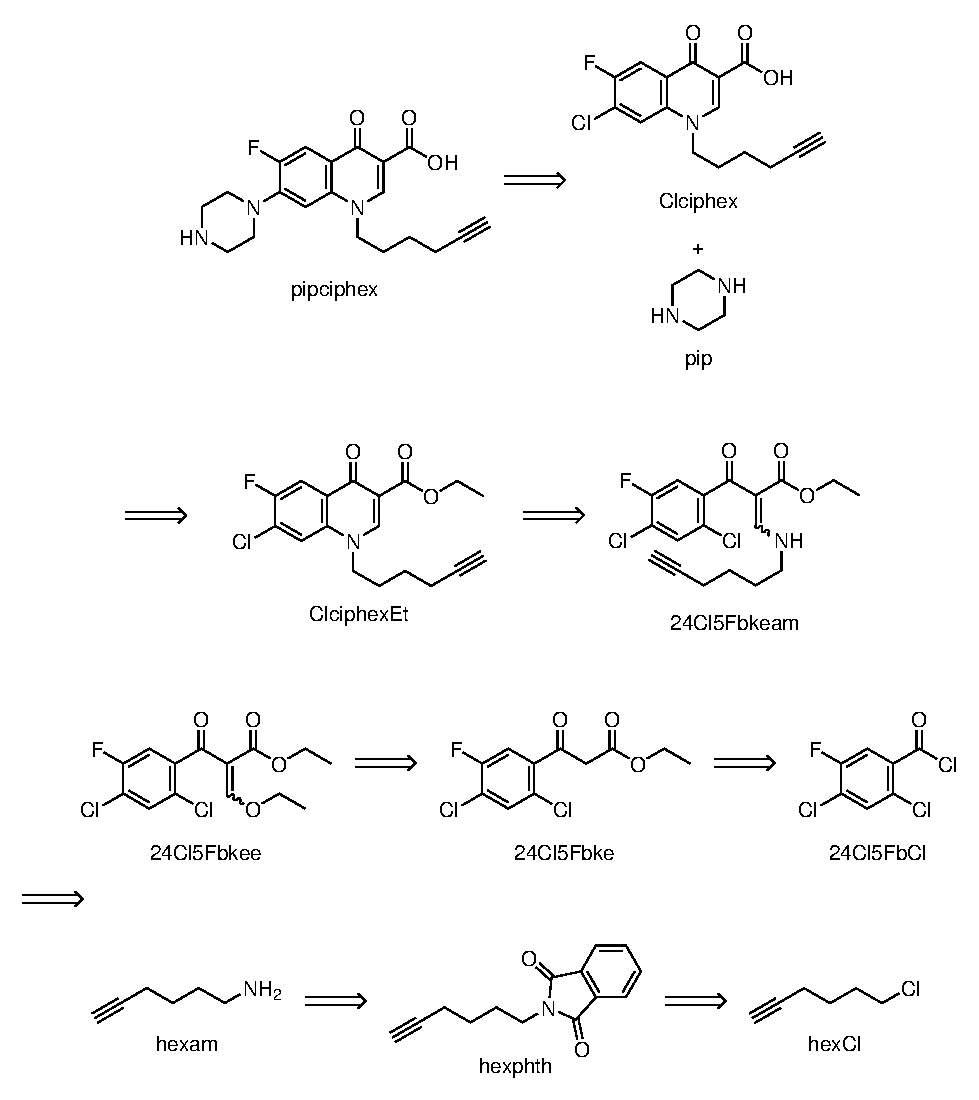
\includegraphics[scale=1]{pipciphex_retro}
%		\caption{The retrosynthesis of \compound{cmpd:pipciphex}. \label{sch:pipciphex_retro}}
%	\end{center}
%\end{scheme}

The initial synthesis of \compound{cmpd:24Cl5Fbke} was attempted using a Claisen condensation and decarboxylation procedure developed by Hanan \textit{et al.}\ \cite{Hanan2012} involving stirring \compound{cmpd:24Cl5FbCl} with potassium ethyl malonate, \ce{MgCl2} and \ce{NEt3}. This procedure had been reported to work using 2-methyl-5-chlorobenzoyl chloride and 2,6-dichlorobenzoyl chloride, however, no reaction was observed using 2,4-dichloro-5-fluorobenzoyl chloride. A modification of the procedure described by Scribner \textit{et al.} \cite{Scribner1978} was used to convert an acid chloride to a $\beta$-ketoester via a Medrum's acid adduct was then attempted. The procedure did produce the desired $\beta$-ketoester \compound{cmpd:24Cl5Fbke}, however, it also produced significant amounts of the ethyl ester \compound{cmpd:24Cl5FbOEt} as a side-product, despite attempts to remove excess acid chloride \compound{cmpd:24Cl5FbCl} before refluxing in ethanol. A modification used by Yamamoto \cite{Yamamoto1987} which substituted pyridine with 4-dimethylaminopyridine also failed to suppress formation of the ethyl ester side product \compound{cmpd:24Cl5FbOEt}. As the product and side-product were relatively difficult to separate by column chromatography, a procedure which did not produce the ethyl ester was sought. 
The \ce{TiCl4}-catalysed crossed Claisen condensation of the acid chloride \compound{cmpd:24Cl5FbCl} and ethyl acetate described by Hashimoto \textit{et al.} \cite{Hashimoto2006} was chosen. This produced the $\beta$-ketoester \compound{cmpd:24Cl5Fbke} without the ethyl ester side product \compound{cmpd:24Cl5FbOEt}.



%\begin{scheme}[H]
%	\begin{center}
%		\schemeref[24Cl5FbCl]{cmpd:24Cl5FbCl}
%		\schemeref[24Cl5Fbke]{cmpd:24Cl5Fbke}
%		\schemeref[24Cl5FbOEt]{cmpd:24Cl5FbOEt}
%		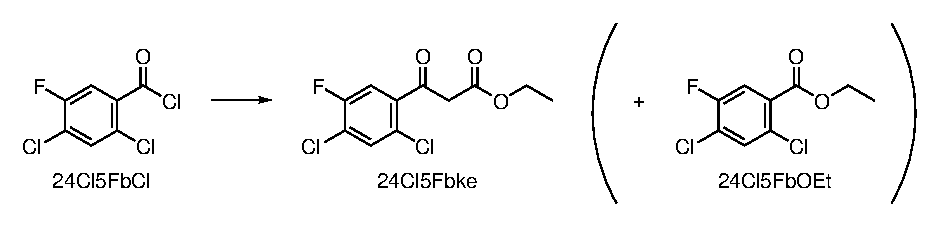
\includegraphics[scale=1]{24Cl5Fbke_opt}
%		\caption{The optimisation of the synthesis of \compound{cmpd:24Cl5Fbke} (see \ref{tbl:24Cl5Fbke_opt}).
%		 \label{sch:24Cl5Fbke_opt}}
%	\end{center}
%\end{scheme}


%\renewcommand{\arraystretch}{1.2}
%\begin{table}[ht]
%  \centering
%\begin{tabular}{|p{0.27\textwidth}|p{0.3\textwidth}|}
%\hline 
%\textbf{Conditions} & \textbf{Outcome} \\ 
%\hline 
%Potassium ethyl malonate \ce{NEt3}, \ce{MgCl2}, MeCN, r.t., 18 h. & No reaction \\ 
%\hline 
%Potassium ethyl malonate \ce{NEt3}, \ce{MgCl2}, r.t., 18 h. & No reaction \\ 
%\hline 
%i) Meldrum's acid, pyridine, \ce{CH2Cl2}, 0 $^{\circ}$C, 4 h. & Product \compound{cmpd:24Cl5Fbke} and side-product \compound{cmpd:24Cl5FbOEt} \\ 
%ii) EtOH, reflux, 18 h. & \\ 
%\hline 
%i) Meldrum's acid, 4-dimethylaminopyridine, \ce{CH2Cl2}, 0 $^{\circ}$C, 4 h. & Product \compound{cmpd:24Cl5Fbke} and side-product \compound{cmpd:24Cl5FbOEt} \\ 
%ii) EtOH, reflux, 18 h. & \\ 
%\hline 
%EtOAc, \ce{TiCl4}, DIPEA, \textit{N}-methyl imidazole, toluene, r.t., 30 min. & Product \compound{cmpd:24Cl5Fbke} \\ 
%\hline 
%\end{tabular}
%\caption{Conditions attempted for the synthesis of \compound{cmpd:24Cl5Fbke} (see \ref{sch:24Cl5Fbke_opt}).\label{tbl:24Cl5Fbke_opt}} 
%\end{table}

The ethoxymethylene group in \compound{cmpd:24Cl5Fbkee} was installed by the reaction of $\beta$-ketoester \compound{cmpd:24Cl5Fbke} and triethyl orthoformate to give a mixture of the \textit{E} and \textit{Z} isomers\cite{Senthilkumar2009,Mitscher1986}.
Hex-5-yn-1-amine \compound{cmpd:hexam} was prepared using a Gabriel synthesis \cite{Gabriel1887} described by Rożkiewicz \textit{et al.} \cite{Rozkiewicz2006}. 6-Chlorohex-1-yne \compound{cmpd:hexCl} was heated with potassium phthalimide to form \compound{cmpd:hexphth}, which was then cleaved using hydrazine monohydrate to form hex-5-yn-1-amine \compound{cmpd:hexam}.
The remainder of the synthesis of \compound{cmpd:pipciphex} is in progress (see \ref{sch:pipciphex_synth}).

\begin{scheme}[H]
	\begin{center}
		\schemeref[24Cl5FbCl]{cmpd:24Cl5FbCl}
		\schemeref[24Cl5Fbke]{cmpd:24Cl5Fbke}
		\schemeref[24Cl5Fbket]{cmpd:24Cl5Fbket}
		\schemeref[24Cl5Fbkee]{cmpd:24Cl5Fbkee}
		\schemeref[hexCl]{cmpd:hexCl}
		\schemeref[hexphth]{cmpd:hexphth}
		\schemeref[hexam]{cmpd:hexam}
		\schemeref[24Cl5Fbkeam]{cmpd:24Cl5Fbkeam}
		\schemeref[ClciphexEt]{cmpd:ClciphexEt}
		\schemeref[Clciphex]{cmpd:Clciphex}
		\schemeref[pip]{cmpd:pip}
		\schemeref[pipciphex]{cmpd:pipciphex}
		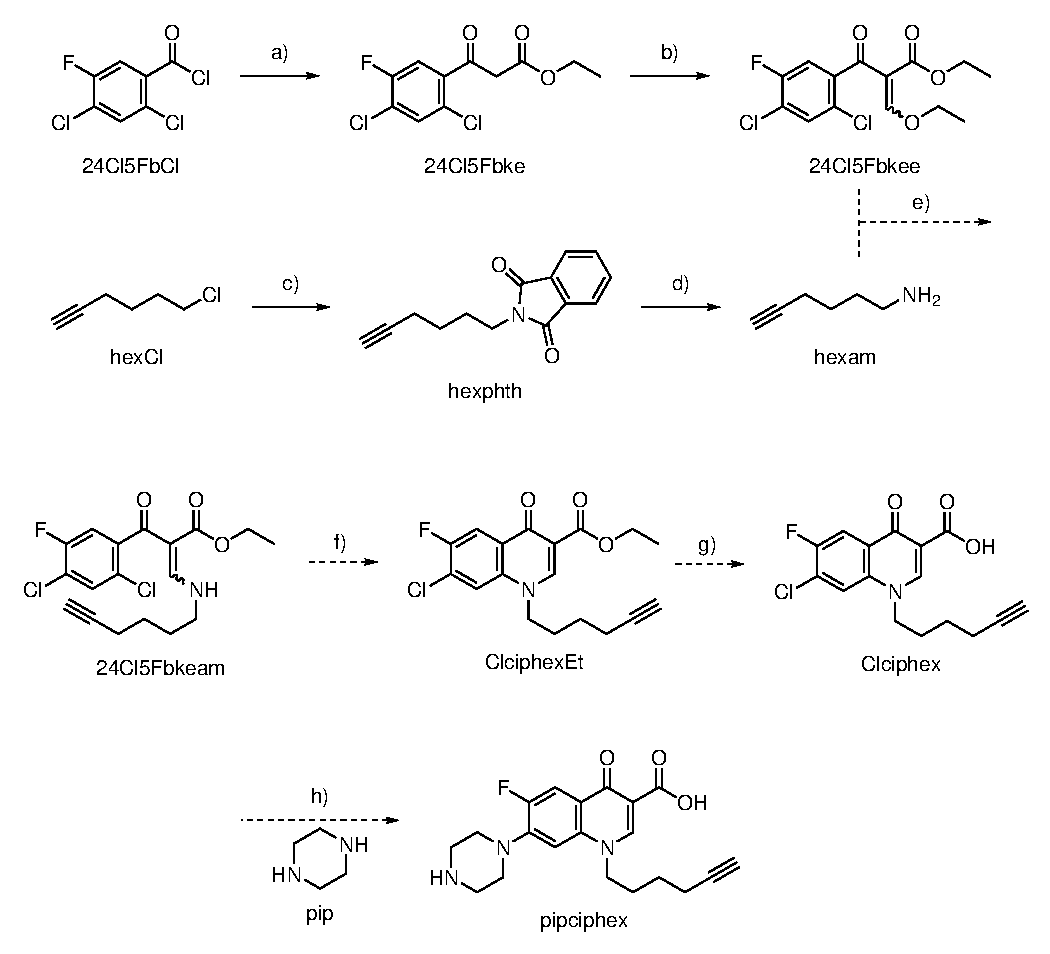
\includegraphics[scale=1]{pipciphex_synth}
		\caption{The synthesis of \compound{cmpd:pipciphex}.
		a) EtOAc, \ce{TiCl4}, DIPEA, \textit{N}-methyl imidazole, toluene, r.t., 30 min, yield \%.
		b) Triethyl orthoformate, \ce{Ac2O}, reflux, 2 h, yield \%.
		c) Potassium phthalimide, KI, DMF, 80 $^{\circ}$C, 18 h, 75 \%.
		d) \ce{N2H2}.\ce{H2O}, EtOH, reflux, 18 h, yield \%.
		e) EtOH.
		f) NaH, dioxane.
		g) KOH, THF.
		h) Piperazine, DMSO.
		\label{sch:pipciphex_synth}}
	\end{center}
\end{scheme}

\subsubsection{Sulfanilamide derivative}

Sulfanilamide antibiotics were the first class to be widely used\cite{Otten1986,Wainwright2011}. The first drug in the class was called Prontosil \compound{cmpd:Pron} and was developed by Bayer and first patented in 1937. Prontosil \compound{cmpd:Pron} is inactive in vitro but active in vivo, as it is a prodrug which is reduced in vivo to release the active drug, sulfanilamide \compound{cmpd:Sul}, and 1,2,4-triaminobenzene \compound{cmpd:124am} (see \ref{fig:Pron}).



\begin{scheme}[H]
	\begin{center}
	\schemeref[Pron]{cmpd:Pron}
	\schemeref[Sul]{cmpd:Sul}
	\schemeref[124am]{cmpd:124am}
		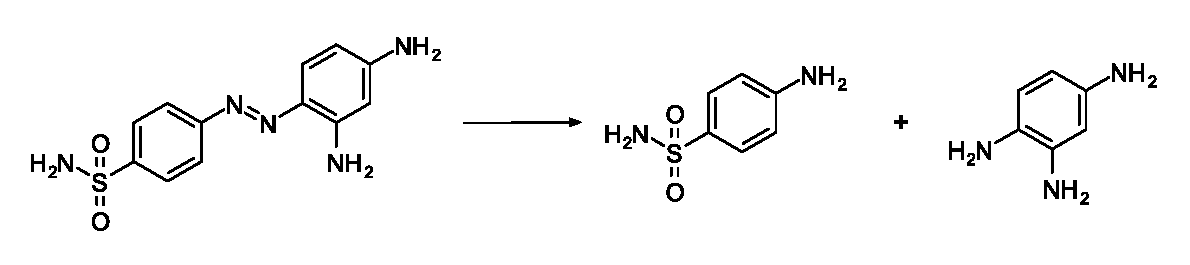
\includegraphics[scale=1]{Pron}
		\caption{The reduction of Prontosil \compound{cmpd:Pron} to release sulfanilamide \compound{cmpd:Sul} and 1,2,4-triaminobenzene \compound{cmpd:124am}.
		\label{fig:Pron}}
	\end{center}
\end{scheme}

Derivatives of sulfaniliamide \compound{cmpd:Sul} have previously been synthesised using a click reaction to append different R groups\cite{Wang2010} (see \ref{sch:Y1Sul_click}). However, if one considers sulfonamide antibiotics already in use, all except sulfacetamide have a heterocycle linked directly to the sulfur atom, rather than with a methylene group in between (see \ref{fig:Sul_ABs}). 

\begin{scheme}[H]
	\begin{center}
		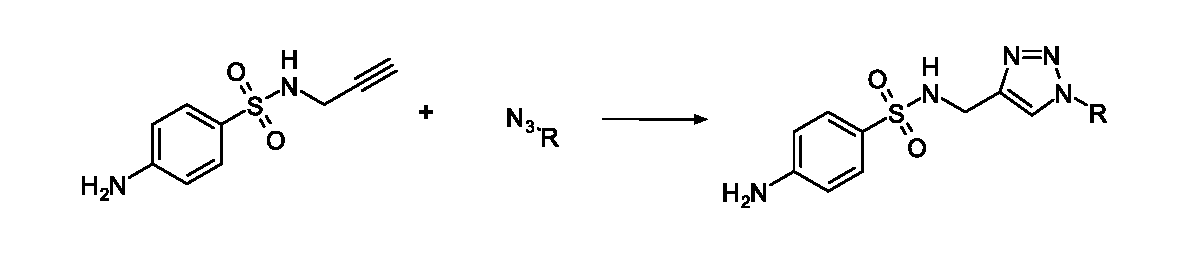
\includegraphics[scale=1]{Y1Sul_click}
		\caption{The sulfanilamide derivatives synthesised using click chemistry by Wang et al\cite{Wang2010}.
		\label{sch:Y1Sul_click}}
	\end{center}
\end{scheme}

\begin{scheme}[H]
	\begin{center}
		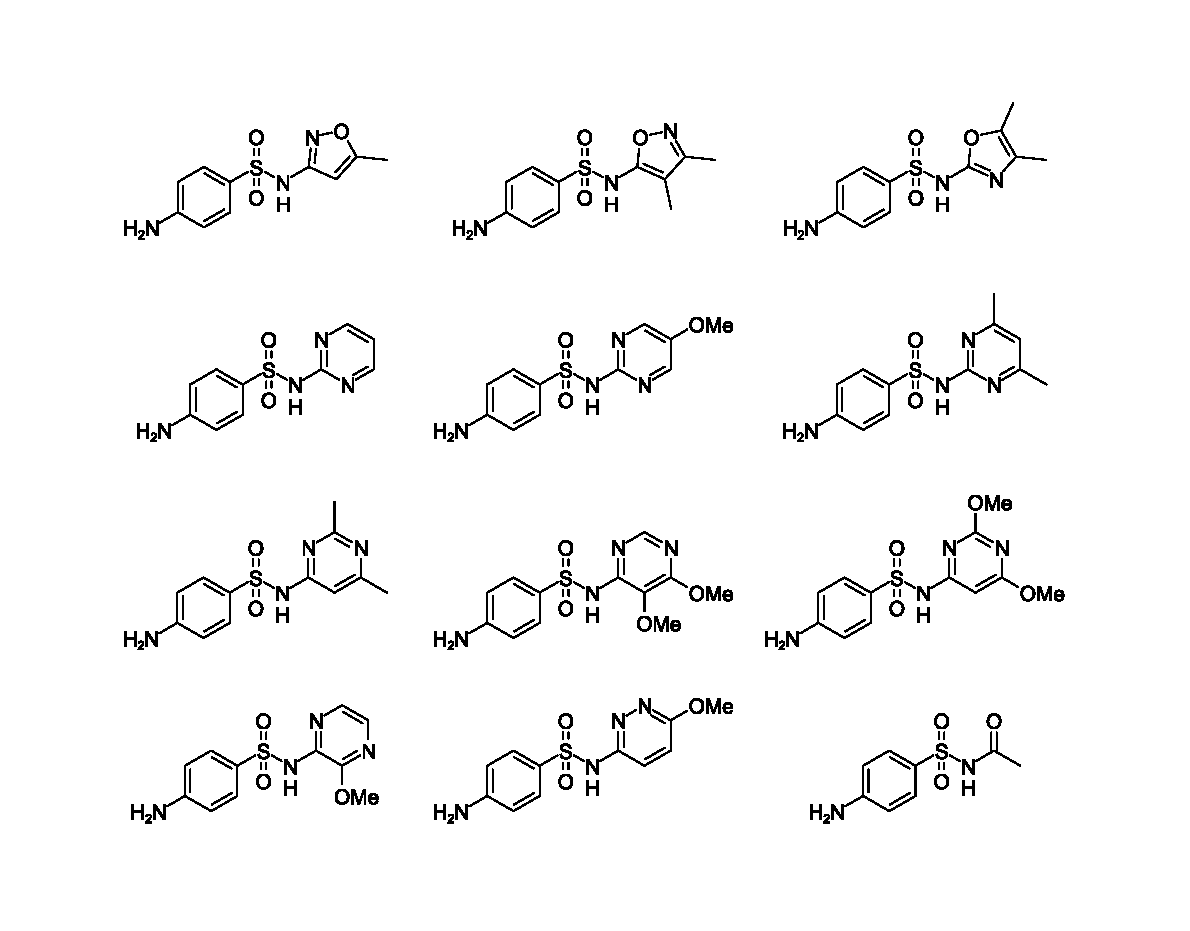
\includegraphics[scale=1]{Sul_ABs}
		\caption{Sulfonamide antibiotics.
		\label{fig:Sul_ABs}}
	\end{center}
\end{scheme}

Therefore, it is postulated that a 1,2,3-triazole could be introduced in the position occupied by a heterocycle in other known sulfonamide antibiotics by attachment of an alkyne directly to the sulfonamide nitrogen to form compound \compound{cmpd:Y0Sul} or a protected version of it (see \ref{sch:Y0Sul_idea}).

\begin{scheme}[H]
	\begin{center}
		\schemeref[Y0Sul]{cmpd:Y0Sul}
		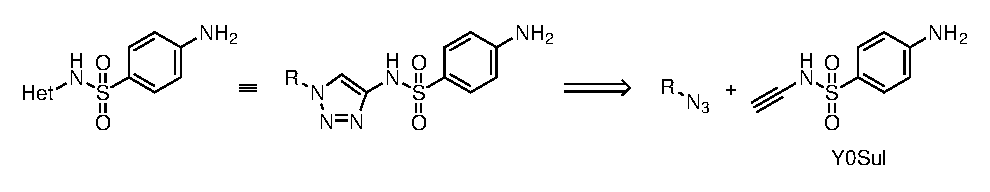
\includegraphics[scale=1]{Y0Sul_idea}
		\caption{Retrosynthesis of a 1,2,3-triazole-containing sulfonamide antibiotic-autoinducer hybrid.
		\label{sch:Y0Sul_idea}}
	\end{center}
\end{scheme}



It is hoped that sulfanilamide derivative \compound{cmpd:Y0Sul} could be synthesised and reacted with the azido autoinducer derivatives directly. This would allow a more efficient synthesis of the library, as no deprotection steps would be needed after the click reaction. However, it appears that no secondary ynamides have been synthesised to date\cite{ScifinderSecondaryYnamide}.
Documents referring to the synthesis of secondary ynamides are either missing \cite{Vellanki2013}, do not refer to the reaction catalogued by Scifinder\cite{Yamaguchi2013,Kaiser2010,Zavyalov1967}, refer compounds containing proparagyl groups instead of ynamides\cite{Gnaccarini2012,Wang2012,Rajopadhye2007,LeitDeMoradeiMarcela2006} or mention unlikely reactions with ethynamine\cite{Edmondson2013} or a derivative\cite{Fujimaki1999} without mentioning how these precursors were synthesised. Scifinder does not have a synthesis of ethynamine, suggesting that it is too unstable to form, but does have two papers discussing the syntheses of other primary ynamines \cite{Shvartsberg1976,Hill1998}.

\begin{scheme}[H]
	\begin{center}
		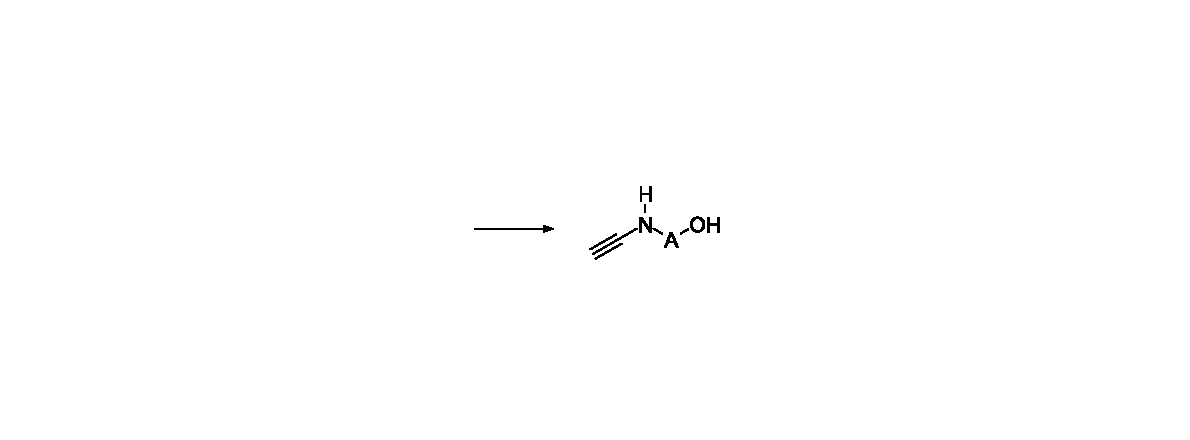
\includegraphics[scale=1]{Scifinder}
		\caption{The Scifinder reaction substructure search used to show that secondary ynamides have not yet been synthesised\cite{ScifinderSecondaryYnamide}.
		\label{fig:Scifinder}}
	\end{center}
\end{scheme}

\begin{scheme}[H]
	\begin{center}
		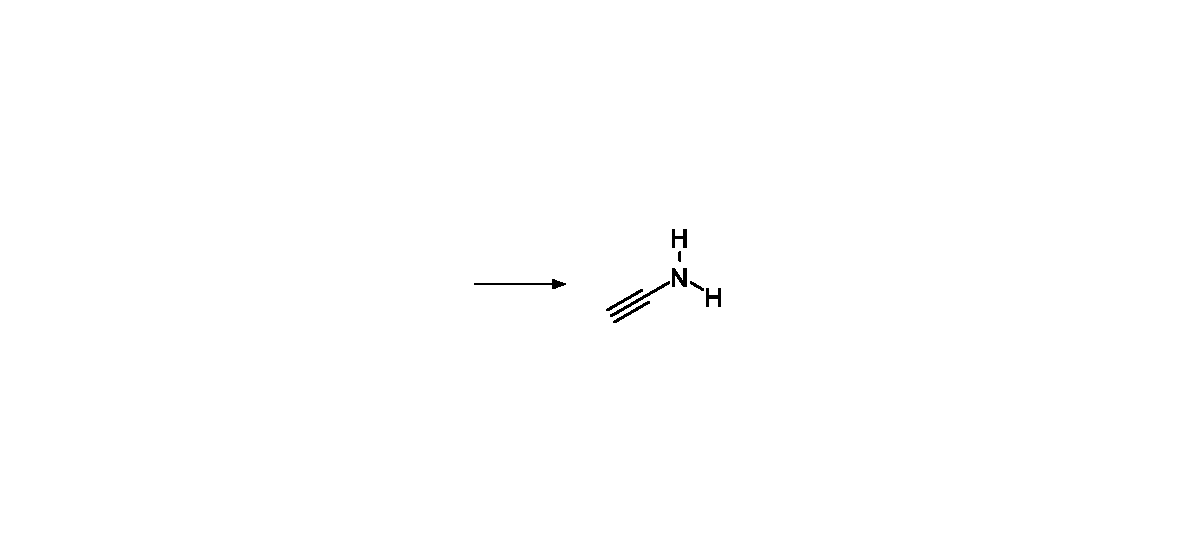
\includegraphics[scale=1]{Scifinder_primary_ynamine}
		\caption{The Scifinder reaction substructure search used to find the synthses of primary ynamines\cite{ScifinderPrimaryYnamine}.
		\label{fig:Scifinder_primary_ynamine}}
	\end{center}
\end{scheme}


Conversely, the synthesis of tertiary ynamines has been studied more widely\cite{Ficini1976}. In particular, tertiary ynamides (often defined as ynamines with any electron-withdrawing group attached) have been shown to be relatively stable and easy to work with in reactions including 
addition at the $\alpha$ position, 
addition at the $\beta$ position, 
reduction/reductive coupling
oxidation,
cycloaddition, 
ring-closing metathesis,
cycloisomerisation,
functionalisation of terminal ynamides and click reactions\cite{IJsselstijn2006,Evano2010}. 

The study of click reactions of ynamides by IJsselstijn et al. uses terminal ynamides protected using a benzyl and a tosyl group or a benzyl and a benzoyl group. Although their click reactions proceed with high yield, they fail to present the deprotection of their final compounds. However, these reactions provide a promising suggestion that click reactions between a protected sulfanilamide derivative and the azido-autoinducer derivatives are feasible. The tosyl group used by IJsselstijn et al. to protect their ynamide is very similar to the \textit{p}-aminobenzenesulfonyl group needed in the alkynyl-sulfanilamide derivative. However, installation of the alkyne could be problematic in the presence of a second amine, so the \ce{NH2} group is installed as a \ce{NO2} group and reduced after the click reaction.  Similarly, the benzyl protecting group must be removed after the click reaction.

%\begin{scheme}[H]
%	\begin{center}
%	\schemeref[PMBa]{cmpd:PMBa}
%	\schemeref[NsCl]{cmpd:NsCl}
%	\schemeref[TIPSY]{cmpd:TIPSY}
%	\schemeref[TIPSYBr]{cmpd:TIPSYBr}
%	\schemeref[NsPMB]{cmpd:NsPMB}
%	\schemeref[TIPSYNsPMB]{cmpd:TIPSYNsPMB}
%	\schemeref[YNsPMB]{cmpd:YNsPMB}
%	\schemeref[HL2N3]{cmpd:HL2N3}
%	\schemeref[HL2TNsPMB]{cmpd:HL2TNsPMB}
%	\schemeref[HL2T0Sul]{cmpd:HL2T0Sul}
%		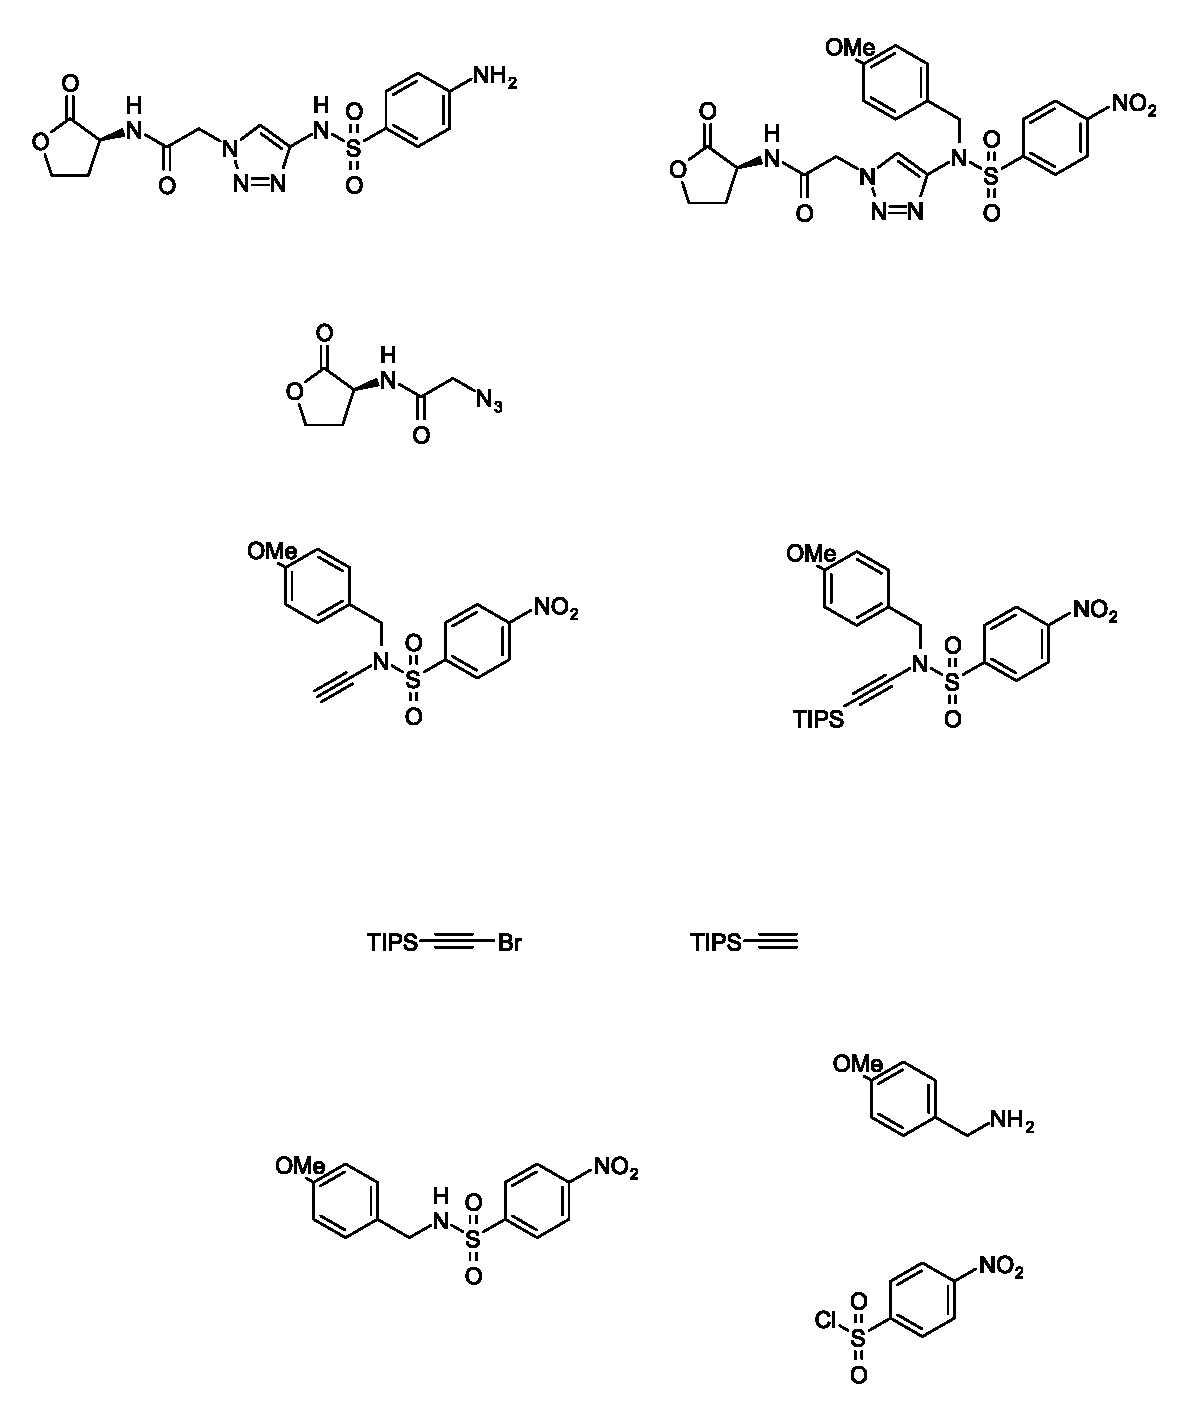
\includegraphics[scale=1]{HL2T0Sul_retro}
%		\caption{Retrosynthesis of a 1,2,3-triazole-containing sulfonamide antibiotic-autoinducer hybrid.
%		\label{sch:HL2T0Sul_retro}}
%	\end{center}
%\end{scheme}



\begin{scheme}[H]
	\begin{center}
	\schemeref[PMBa]{cmpd:PMBa}
	\schemeref[NsCl]{cmpd:NsCl}
	\schemeref[TIPSY]{cmpd:TIPSY}
	\schemeref[TIPSYBr]{cmpd:TIPSYBr}
	\schemeref[NsPMB]{cmpd:NsPMB}
	\schemeref[TIPSYNsPMB]{cmpd:TIPSYNsPMB}
	\schemeref[YNsPMB]{cmpd:YNsPMB}
	\schemeref[HL2N3]{cmpd:HL2N3}
	\schemeref[HL2TNsPMB]{cmpd:HL2TNsPMB}
	\schemeref[HL2T0Sul]{cmpd:HL2T0Sul}
		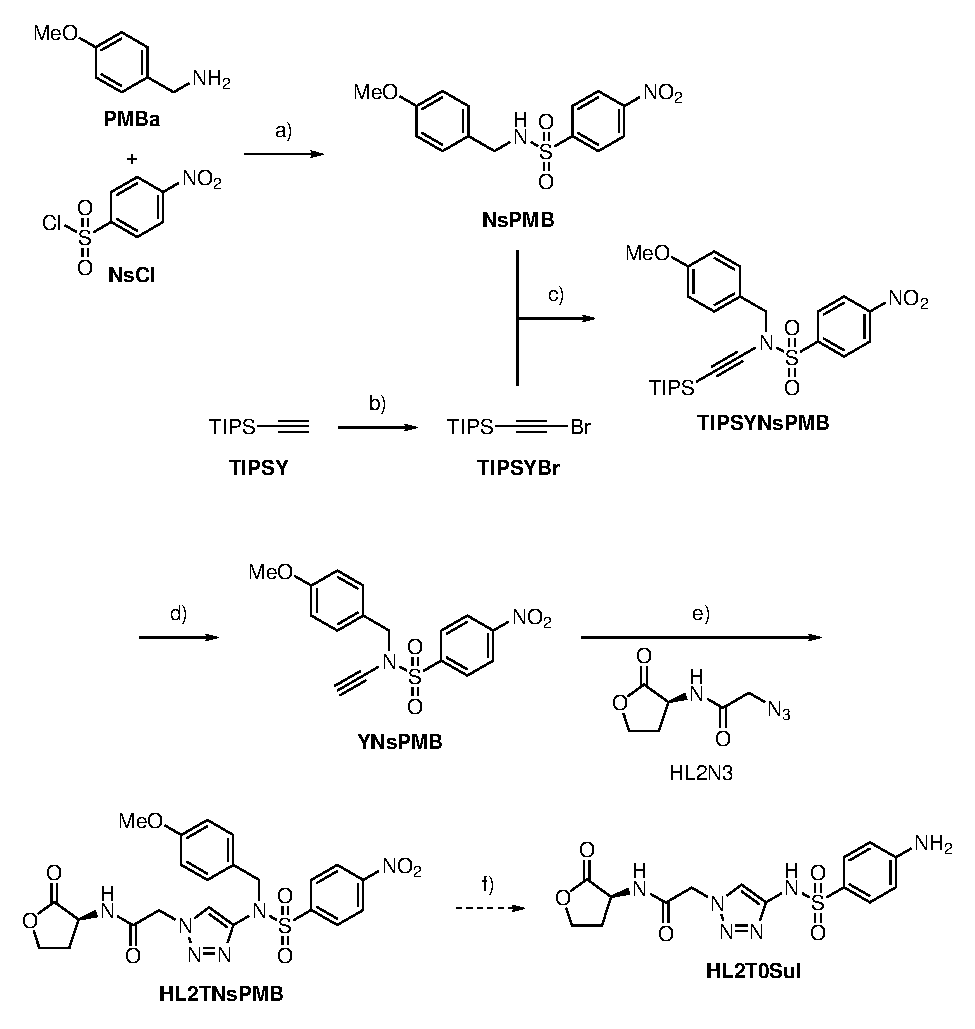
\includegraphics[scale=1]{HL2T0Sul_synth}
		\caption{Synthesis of a 1,2,3-triazole-containing sulfonamide antibiotic-autoinducer hybrid.
		a) \ce{CH2Cl2}, r.t., 24 h \cite{Bendikov2005}. 
		b) \ce{AgNO3}, acetone, r.t., 3 h \cite{Graux2014}. 
		c) \ce{CuSO4.5H2O}, 1,10-phenanthroline, \ce{K2CO3}, toluene, $80\ ^{\circ}$C, 48 h \cite{Graux2014}. 
		d) TBAF, THF, $-78\ ^{\circ}$C, 3 h\cite{Graux2014}. 
		e) \ce{Cu(OAc)2}, sodium ascorbate, \ce{CH2Cl2}, \textit{t}-BuOH, \ce{H2O}, r.t., 16 h \cite{IJsselstijn2006}. 
		f) \ce{SnCl2}, TFA, \ce{CH2Cl2}, reflux, 3 h \cite{Bissinger2011, Reuillon2012}.
		\label{sch:HL2T0Sul_synth}}
	\end{center}
\end{scheme}

%\subsubsection{Retrosynthesis of sulfanilimide derivatives \compound{cmpd:Y1Sul} and \compound{cmpd:Y4Sul}}

\subsubsection{Linezolid derivative}

If time permits, an alkynyl derivative of the antibiotic linezolid \compound{cmpd:Lin} (see \ref{fgr:ABs}) could also be synthesised. The route follows a recent literature procedure described by Phetsang \textit{et al}.\cite{Phetsang2014}. The morpholine ring of linezolid is replaced by piperazine, allowing an alkynyl tail to be attached to the molecule (as opposed to the azido tail attached by Phetsang \textit{et al}.).

%\begin{scheme}[H]
%	\begin{center}
%		\schemeref[2FN]{cmpd:2FN}
%		\schemeref[Pip]{cmpd:Pip}
%		\schemeref[PipFN]{cmpd:PipFN}
%		\schemeref[PipFAm]{cmpd:PipFAm}
%		\schemeref[CbzPipFAmCbz]{cmpd:CbzPipFAmCbz}
%		\schemeref[RGlyBu]{cmpd:RGlyBu}
%		\schemeref[CbzPipFOxaOH]{cmpd:CbzPipFOxaOH}
%		\schemeref[CbzPipFOxaOTs]{cmpd:CbzPipFOxaOTs}
%		\schemeref[KPhth]{cmpd:KPhth}
%		\schemeref[CbzPipFOxaPhth]{cmpd:CbzPipFOxaPhth}
%		\schemeref[CbzPipFOxaAm]{cmpd:CbzPipFOxaAm}
%		\schemeref[CbzPipFOxaAmAc]{cmpd:CbzPipFOxaAmAc}
%		\schemeref[PipFOxaAmAc]{cmpd:PipFOxaAmAc}
%		\schemeref[Y4I]{cmpd:Y4I}
%		\schemeref[Y4PipFOxaAmAc]{cmpd:Y4PipFOxaAmAc}
%		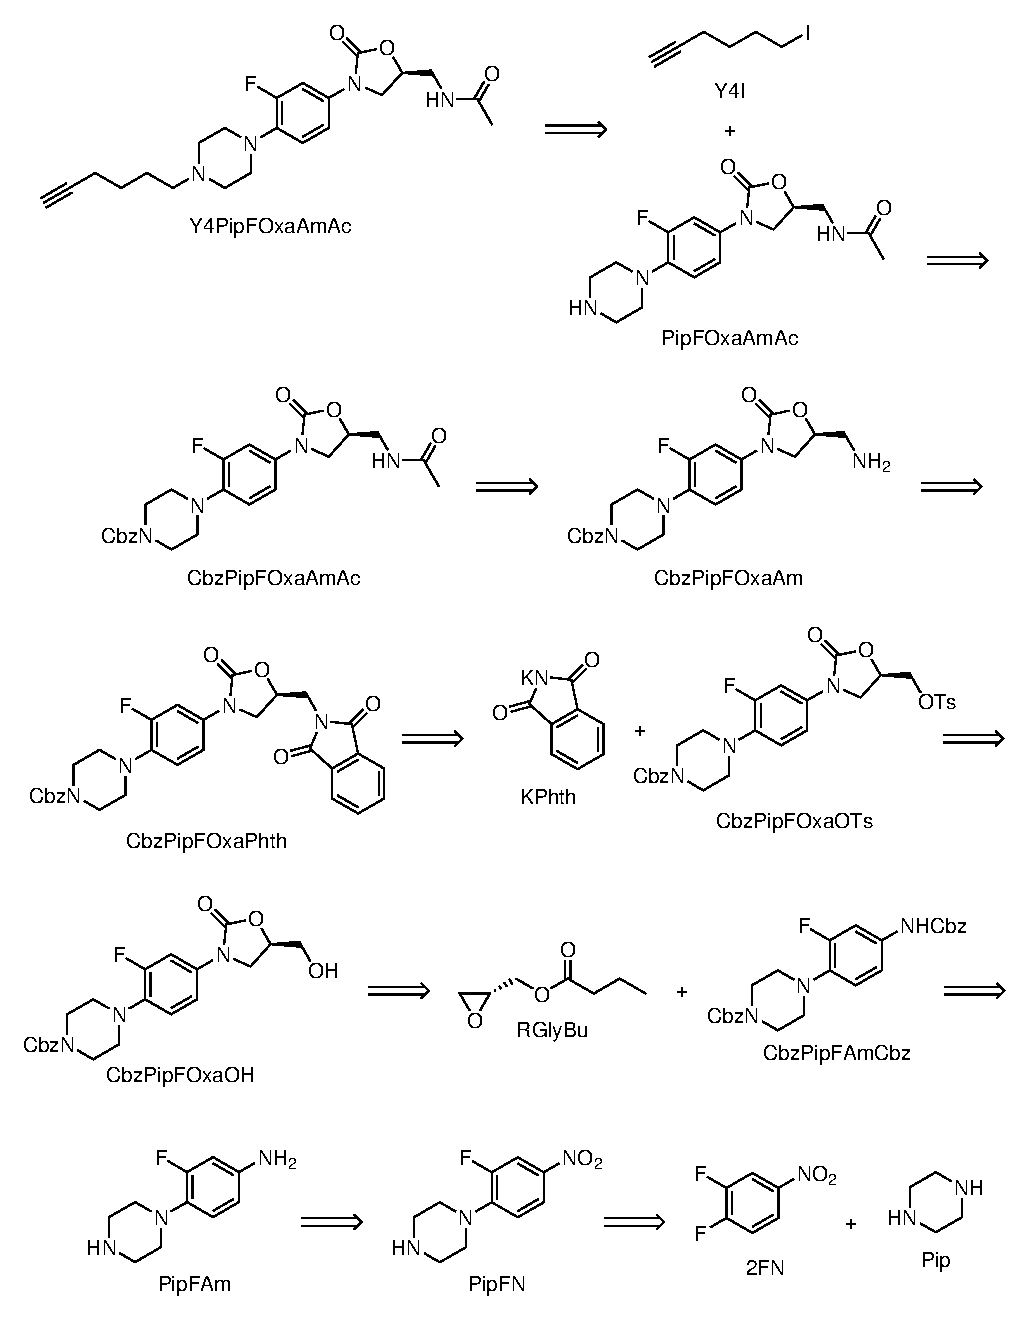
\includegraphics[scale=1]{YLin_retro}
%		\caption{Retrosynthesis of linezolid derivative \compound{cmpd:YLin}\cite{Phetsang2014}.
%		\label{sch:YLin_retro}}
%	\end{center}
%\end{scheme}


\begin{scheme}[H]
	\begin{center}
		\schemeref[2FN]{cmpd:2FN}
		\schemeref[Pip]{cmpd:pip}
		\schemeref[PipFN]{cmpd:PipFN}
		\schemeref[PipFAm]{cmpd:PipFAm}
		\schemeref[CbzPipFAmCbz]{cmpd:CbzPipFAmCbz}
		\schemeref[RGlyBu]{cmpd:RGlyBu}
		\schemeref[CbzPipFOxaOH]{cmpd:CbzPipFOxaOH}
		\schemeref[CbzPipFOxaOTs]{cmpd:CbzPipFOxaOTs}
		\schemeref[KPhth]{cmpd:KPhth}
		\schemeref[CbzPipFOxaPhth]{cmpd:CbzPipFOxaPhth}
		\schemeref[CbzPipFOxaAm]{cmpd:CbzPipFOxaAm}
		\schemeref[CbzPipFOxaAmAc]{cmpd:CbzPipFOxaAmAc}
		\schemeref[PipFOxaAmAc]{cmpd:PipFOxaAmAc}
		\schemeref[Y4I]{cmpd:Y4I}
		\schemeref[Y4PipFOxaAmAc]{cmpd:Y4PipFOxaAmAc}
		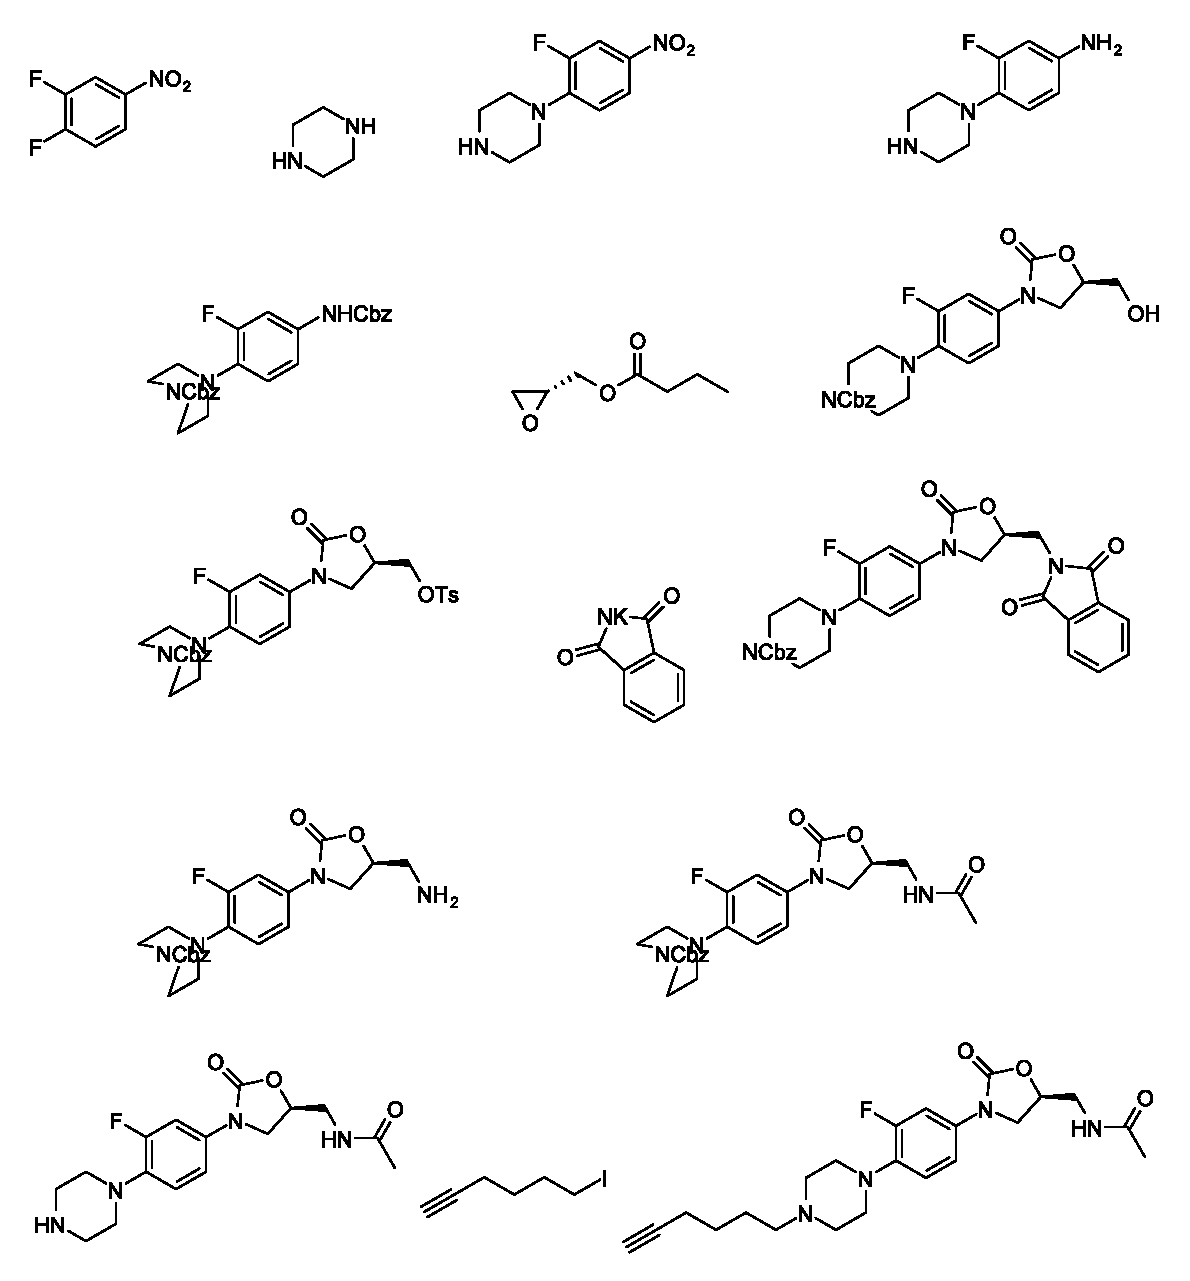
\includegraphics[scale=1]{YLin_synth}
		\caption{Proposed synthesis of linezolid derivative \compound{cmpd:YLin}\cite{Phetsang2014}.
		a) MeCN, reflux, 3 h. 
		b) \ce{H2}, 10 \% Pd/C, THF, 40 psi, <50 $\ ^{\circ}$C, 1.5 h. 
		c) CbzCl, \ce{Na2CO3}, acetone/\ce{H2O}, 1 h at 5 $\ ^{\circ}$C then 16 h at rt. 
		d) \textit{n}-BuLi, THF, -78 $\ ^{\circ}$C for 1 h then add epoxide then -78 $\ ^{\circ}$C for 1.5 h then rt for 3.5 h. 
		e) TsCl, \ce{NEt3}, \ce{CH2Cl2}, 0 $\ ^{\circ}$C for 1.5 h then rt for 3 h. 
		f) MeCN/\ce{H2O}, reflux, 48 h. 
		g) \ce{MeNH2}, EtOH/\ce{H2O}, reflux, 5.5 h. 
		h) \ce{Ac2O}, pyridine, 0 $\ ^{\circ}$C to rt. 
		i) \ce{H2}, 10 \% Pd/C, MeOH/\ce{CH2Cl2}, 1 atm, rt, 16 h. 
		j) \ce{NEt3}, EtOH, reflux.%, 6 h.
		\label{sch:YLin_synth}}
	\end{center}
\end{scheme}



\subsubsection{Penicillin derivative \compound{cmpd:hexpen}\label{sec:Futpen}}

The penicillins are a group of antibiotics with the same penam core structure but different R groups (see \ref{fgr:pen_anas}). It therefore seems likely that a biologically active penicillin derivative could be synthesised with an alkyne in the R group. This could be produced using the penicillin precursor 6-aminopenicillanic acid \compound{cmpd:6APA} and 5-hexynoic acid \compound{cmpd:hexOOH} or a derivative thereof. 
An initial attempt at synthesis was based on a procedure developed by Faridoon \cite{Faridoon2012}. Firstly, 5-hexynoic acid \compound{cmpd:hexOOH} was converted to 5-hexanoyl chloride \compound{cmpd:hexOCl} using oxalyl chloride and catalytic DMF, unlike in the Faridoon procedure which uses thionyl chloride. 5-hexanoyl chloride \compound{cmpd:hexOCl} was then stirred with 6-aminopenicillanic acid \compound{cmpd:6APA}, however, despite screening various solvent systems and bases no clean reaction could be found and the reactions gave complex mixtures of products. It appears that 6-aminopenicillanic acid \compound{cmpd:6APA} and its derivatives are too sensitive to basic conditions for these conditions to be used, most likely due to opening of the $\beta$-lactam ring followed by further decomposition reactions. Products were also seen to undergo methanolysis  during \ce{SiO2} column chromatography using \ce{CH2Cl2}/MeOH solvent systems. Therefore, milder reaction conditions must used. Peptide coupling reagents may be useful for this purpose, for example DCC and HOBt (see \ref{sch:hexpen_synth_fut}).


\begin{figure}[H]
	\begin{center}
		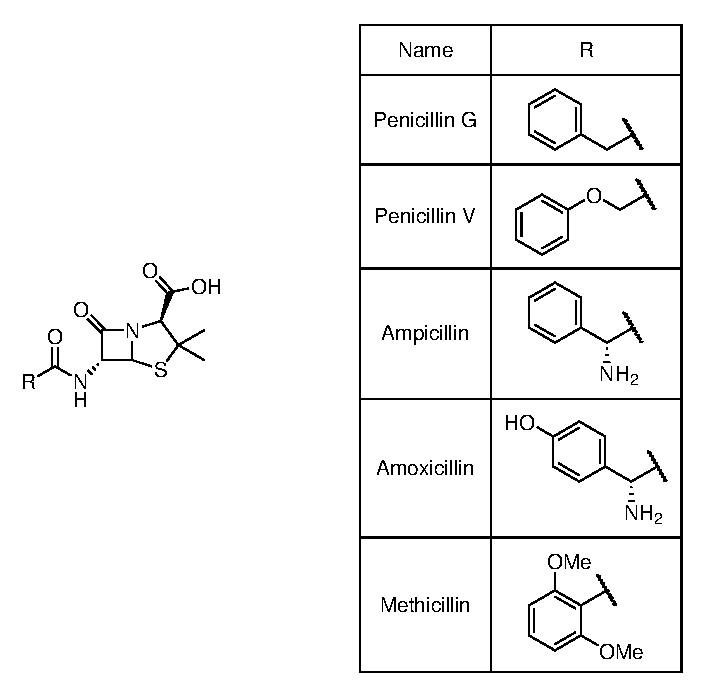
\includegraphics[scale=1]{pen_anas}
		\caption{The penicillins.\label{fgr:pen_anas}} 
	\end{center}
\end{figure}

%\renewcommand{\arraystretch}{1.2}
%\begin{table}[ht]
%  \centering
%\begin{tabular}{|p{0.3\textwidth}|p{0.3\textwidth}|}
%\hline 
%\textbf{Conditions} & \textbf{Outcome} \\ 
%\hline 
%\ce{CH2Cl2}, DIPEA, r.t., 18 h. & Complex mixture \\ 
%\hline
%Pyridine, r.t., 18 h. & Complex mixture \\ 
%\hline
%Acetone/\ce{H2O}, \ce{NaHCO3}, r.t., 18 h. & Complex mixture \\ 
%\hline
%\ce{CH2Cl2}/\ce{H2O}, \ce{NaHCO3}, r.t., 18 h. & Complex mixture \\ 
%\hline 
%\end{tabular}
%\caption{Conditions attempted for the synthesis of \compound{cmpd:hexpen} (see \ref{sch:hexpen_synth})\label{tbl:hexpen_opt}} 
%\end{table}

\begin{scheme}[H]
	\begin{center}
		\schemeref[hexOOH]{cmpd:hexOOH}
		\schemeref[hexOCl]{cmpd:hexOCl}
		\schemeref[6APA]{cmpd:6APA}
		\schemeref[hexpen]{cmpd:hexpen}
		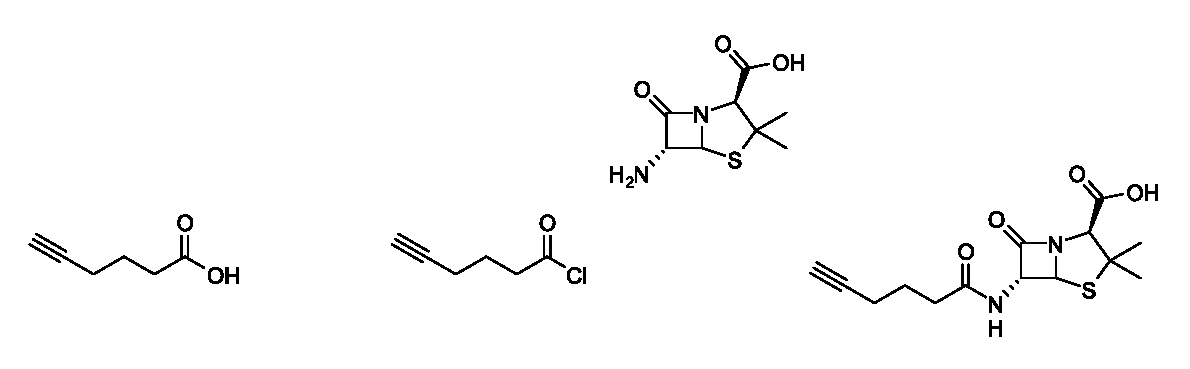
\includegraphics[scale=1]{hexpen_synth}
		\caption{Attempted synthesis of \compound{cmpd:hexpen}. a) oxalyl chloride, DMF, \ce{CH2Cl2}, r.t., 3 h. 
		b) DIPEA, \ce{CH2Cl2}/pyridine/\ce{NaHCO3}, Acetone, \ce{H2O}/\ce{NaHCO3}, \ce{CH2Cl2}, \ce{H2O}, all r.t., 18 h. 
		\label{sch:hexpen_synth}}
	\end{center}
\end{scheme}



\begin{scheme}[H]
	\begin{center}
		\schemeref[hexOOH]{cmpd:hexOOH}
		\schemeref[6APA]{cmpd:6APA}
		\schemeref[hexpen]{cmpd:hexpen}
		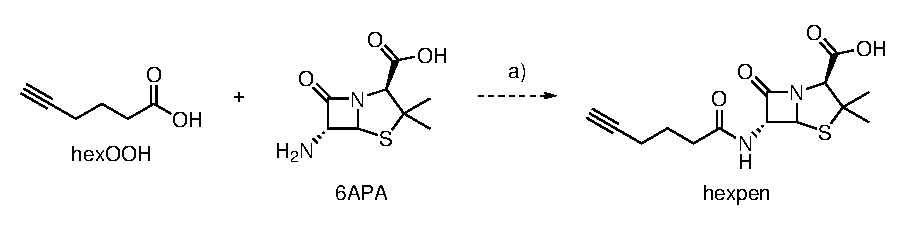
\includegraphics[scale=1]{hexpen_synth_fut}
		\caption{Proposed synthesis of \compound{cmpd:hexpen}. a) DCC, HOBt, DMF. \label{sch:hexpen_synth_fut}}
	\end{center}
\end{scheme}

\subsubsection{Gentamicin derivative \compound{cmpd:hexC1a}}

Gentamicin is an aminoglycoside antibiotic used to treat many bacterial infections, particularly those caused by Gram-negative organisms, by binding to the bacterial ribosome. Gentamicin is actually a mixture of components (see \ref{fgr:gen_anas}) synthesised by \textit{Micromonospora sp.}, a genus of Gram-positive bacteria. Separation of the gentamicin components has been achieved by Grote \textit{et al.} \cite{Grote2012} by reaction with benzyl chloroformate followed by HPLC and hydrogenolysis of the protecting groups. 
Gentamicin C1a \compound{cmpd:C1a} was isolated pure, and is particularly useful because it the only component which contains a \ce{CH2NH2} group. This group is less hindered than all other amine groups in gentamicin C1a \compound{cmpd:C1a} and hence it is possible to selectively derivatise the molecule at this position. Grote \textit{et al.} attached a tag needed for an immunoassay using a pentafluorophenyl ester\cite{Cheshev2010}. Hence, it may be possible to achieve selective reaction of this site with the pentafluorophenyl ester of 5-hexynoic acid \compound{cmpd:hexOOpf} (see \ref{sch:hexC1a_synth}). It may even be possible to react the original gentamicin mixture with the pentafluorophenyl ester and then separate out the desired component.

\begin{figure}[H]
	\begin{center}
		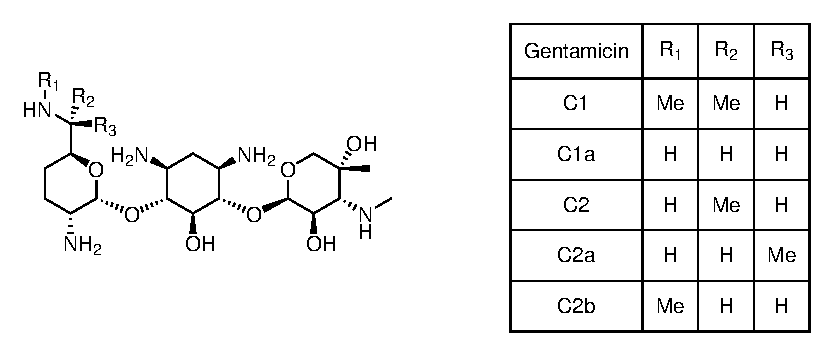
\includegraphics[scale=1]{gen_anas}
		\caption{Gentamicin components. \label{fgr:gen_anas}} 
	\end{center}
\end{figure}

\begin{scheme}[H]
	\begin{center}
		\schemeref[hexOOpf]{cmpd:hexOOpf}
		\schemeref[C1a]{cmpd:C1a}
		\schemeref[hexC1a]{cmpd:hexC1a}
		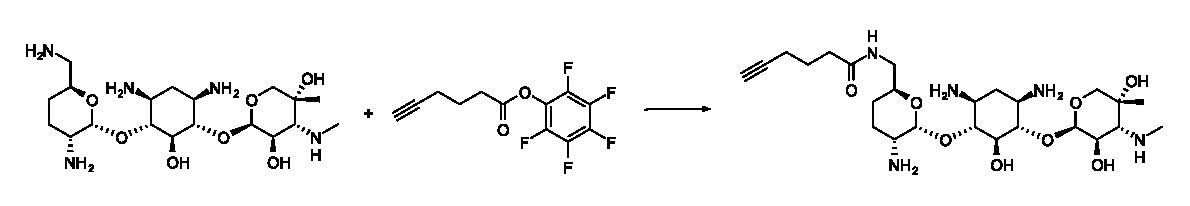
\includegraphics[scale=1]{hexC1a_synth}
		\caption{Proposed synthesis of gentamicin C1a derivative \compound{cmpd:hexC1a}. a) DIPEA, DMF, - 55 $^{\circ}$C. \label{sch:hexC1a_synth}}
	\end{center}
\end{scheme}

\subsubsection{Streptomycin derivatives \compound{cmpd:alkyneOHstr}, \compound{cmpd:redamalkyneNstr} and \compound{cmpd:alkyneNstr}}

Streptopmycin \compound{cmpd:str} is an aminoglycoside antibiotic used to treat \ce{Mycobacterium tuberculosis} and \ce{S. aureus} by binding to the bacterial ribosome. There is limited SAR data on streptomycin but it is known that conversion of the aldehyde to a carboxylic acid destroys activity, whereas conversion an alcohol retains it \cite{lemke2012foye}. TMS protection followed by attack with lithium acetylide then deprotection could be used to produce an derivative \compound{cmpd:alkyneOHstr} with a secondary alcohol in place of the aldehyde (see \ref{sch:alkyneOHstr_synth}).

Reductive amination could also be used to install an alkyne group by reaction of the aldehyde with amino-1-propyne (see \ref{sch:redamalkyneNstr_synth})\cite{Abdel-Magid1996}. This would install NH in place of the aldehyde O; it is known that an OH is tolerated at this position so it seems possible that NH would be as well.

There is one primary alcohol in streptopmycin \compound{cmpd:str} which could be selectively displaced to install an alkyne. Selective displacement could be achieved by reaction with 1 eq. of trifluoroacetic anhydride followed by displacement with amino-1-propyne (see \ref{sch:alkyneNstr_synth})\cite{Coimbra2010}. This leaves an H-bond donor in that position as OH is replaced by NH.


\begin{scheme}[H]
	\begin{center}
		\schemeref[str]{cmpd:str}
		\schemeref[TMSstr]{cmpd:TMSstr}
		\schemeref[TMSalkyneOHstr]{cmpd:TMSalkyneOHstr}
		\schemeref[alkyneOHstr]{cmpd:alkyneOHstr}
		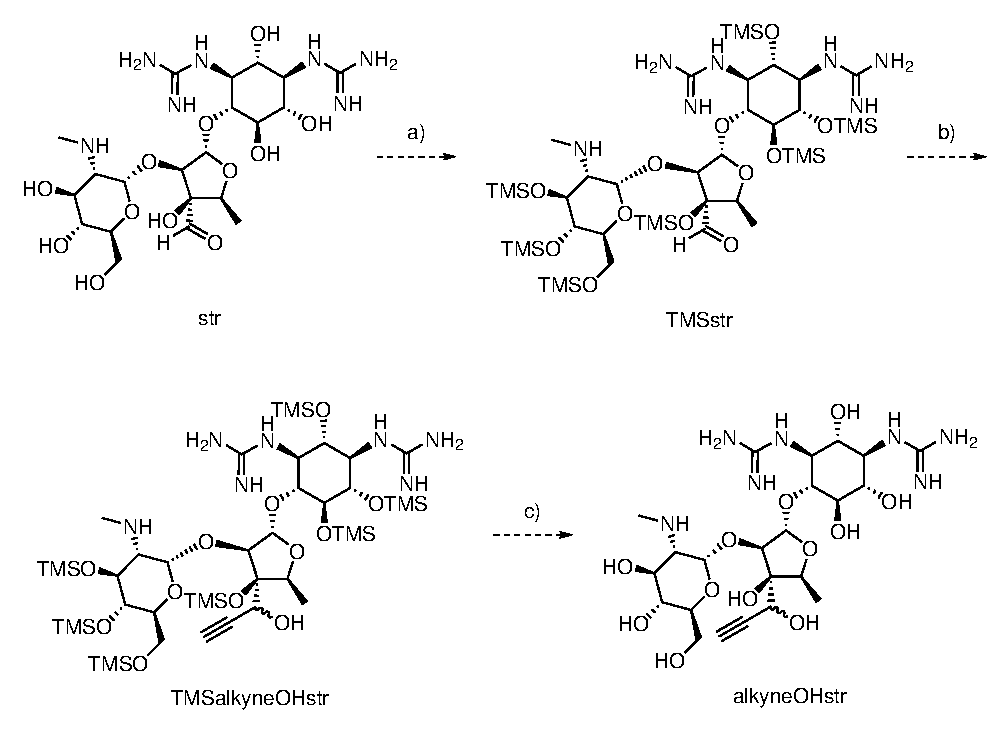
\includegraphics[scale=1]{alkyneOHstr_synth}
		\caption{Proposed synthesis of streptomycin derivative \compound{cmpd:alkyneOHstr}. a) TMSCl. b) Lithium acetylide. c) TBAF. \label{sch:alkyneOHstr_synth}}
	\end{center}
\end{scheme}

\begin{scheme}[H]
	\begin{center}
		\schemeref[str]{cmpd:str}
		\schemeref[alkyneam]{cmpd:alkyneam}
		\schemeref[redamalkyneNstr]{cmpd:redamalkyneNstr}
		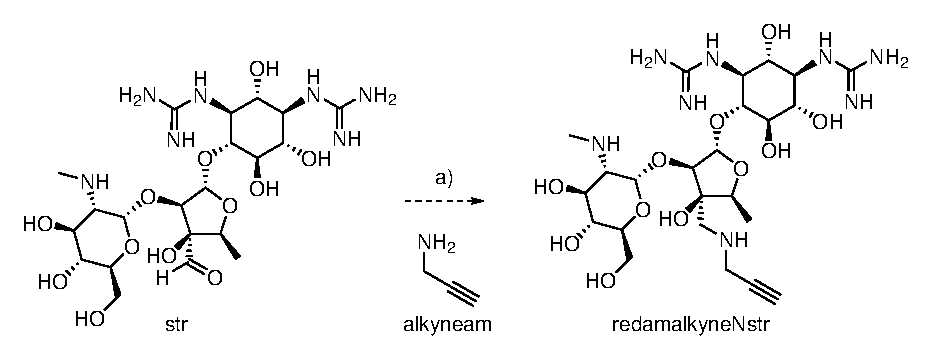
\includegraphics[scale=1]{redamalkyneNstr_synth}
		\caption{Proposed synthesis of streptomycin derivative \compound{cmpd:redamalkyneNstr}. 
		a) \ce{NaBH(AcO)3}, 1,2-dichloroethane, r.t.
		\label{sch:redamalkyneNstr_synth}}
	\end{center}
\end{scheme}

\begin{scheme}[H]
	\begin{center}
		\schemeref[str]{cmpd:str}
		\schemeref[Msstr]{cmpd:Msstr}
		\schemeref[alkyneam]{cmpd:alkyneam}
		\schemeref[alkyneNstr]{cmpd:alkyneNstr}
		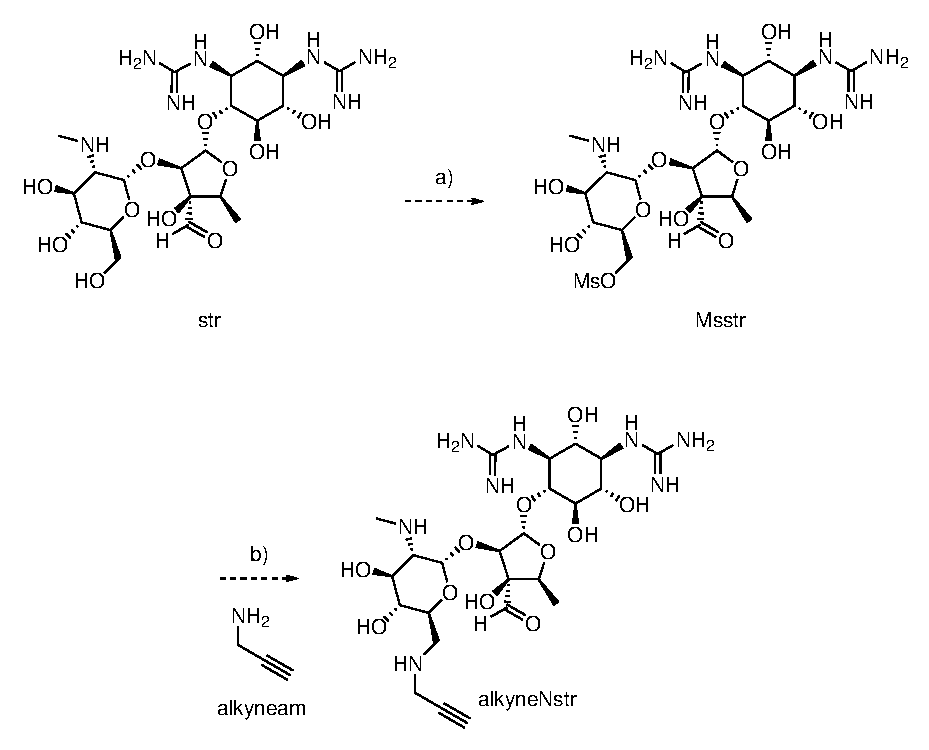
\includegraphics[scale=1]{alkyneNstr_synth}
		\caption{Proposed synthesis of streptomycin derivative \compound{cmpd:alkyneNstr}. 
		a) MsCl, pyridine, \ce{CH2Cl2}, 0 $^{\circ}$C to r.t. 
		b) 3-amino-1-propyne, EtOH.
		\label{sch:alkyneNstr_synth}}
	\end{center}
\end{scheme}

\subsection{Autoinducer analogue derivatives}

\subsection{Linkers}

\subsection{Biology}